%% Template for MLP Coursework 2 / 6 November 2017

%% Based on  LaTeX template for ICML 2017 - example_paper.tex at
%%  https://2017.icml.cc/Conferences/2017/StyleAuthorInstructions

\documentclass{article}
\input{mlp2018_includes}


%% You probably do not need to change anything above this comment

%% REPLACE this with your student number
\def\studentNumber{s1837504}
\usepackage{epstopdf}
\usepackage[toc,page]{appendix}
\begin{document}

\twocolumn[

\mlptitle{An open-data approach to creating bus routes}

\centerline{\studentNumber}

\vskip 7mm
]

\begin{abstract}
As the amount of available data increases so do the opportunities of approaching old problems from a different viewpoint. Our paper tests a novel approach in creating bus routes based on open-data, using taxi trips in Manhattan. After building a bus transportation network we compare its performance to taxis and find that on average it requires 18 more minutes  to complete a journey.
\end{abstract}

\section{Introduction}
No one can deny that the comfort and speed of private transportation is desirable especially when compared to the clustered and slow public transportation. However, considering the effects of $CO_2$ emissions to our environment \citep{schelling_economics_1992} we must find ways to incentivise the use of public transportation. This paper proposes a new approach to automatically create bus routes and compares its performance to taxis in an effort to explore methods which may decrease the duration of bus trips. By utilising open data in the form of 1,509,036 taxi trips in Manhattan \citep{donovan_new_2016}, and the map of Manhattan \citep{openstreetmap_contributors_planet_2018}, we place bus stops and create routes to serve the demand. Our method assumes uncapacitated buses, zero waiting time at bus stops, and achieves a 37\% performance compared to taxis. Our findings also indicate that using $k$-means clustering as a way to grouping stops is a bottleneck in creating efficient routes.

\section{Background}
%The problem of creating bus routes consists of two sub-problems, first we have to determine the bus stops, a facility location problem, and then define the route for each bus, a vehicle routing problem. However, it was shown that solving each problem separately may lead to suboptimal results \citep{salhi_effect_1989}. Therefore, a new family of problems called location-routing problems (LRP) was created. LRPs tackle the facility location problem, i.e. bus stops, while taking into account the vehicle routing problem (VRP) \citep{nagy_location-routing:_2007}. According to \citet{drexl_survey_2015}, the majority of the literature deals with discrete facility locations where the facilities are placed in a subset of given nodes, something which doesn't apply to bus stops. They cite \citet{salhi_local_2009} as the only research related to finding multiple facilities in a continuous grid, a research which yielded only 1.63\% improvement over the classical, separate, approach. As a result of the limited improvements, and the increased difficulty in solving LRPs \citep[p. 431]{drezner_facility_1995}, we choose to solve the two subproblems separately.

The problem of creating bus routes consists of two sub-problems, first we have to determine the bus stops, a facility location problem, and then define the route for each bus, a vehicle routing problem (VRP). Since we do not take into account the cost of opening a bus stop, if we define the number of stops then our facility location problem can be further simplified to a $k$-means problem. The objective is to minimise the sum of squared differences from each point to the cluster's centre and one of the most popular \citep{ostrovsky_effectiveness_2006} approximation algorithms is Lloyd's heuristic \citep{lloyd_least_1982} (see Algorithm~\ref{alg:lloyd}). Two possible centroid initialisations are the "furthest traversal", where the centres are chosen to be far apart, and another strategy is choosing as our starting centres the output of another clustering algorithm \citep[p. 214]{blum_foundations_2018}. In addition, a drawback of "furthest traversal" is that outliers may hinder its performance, an issue that gave birth to $k$-means++ which calculates the initial centres iteratively with probability proportional to the square distance from the closest, already selected, centre \citep{arthur_k-means++:_2007}. A more appropriate formulation, since we have a grid, would be to create a $k$-median problem which minimises the error with respect to the $L^1$ norm. However, the magnitude of our data requires an efficient implementation and the $k$-means method provided by scikit-learn \citep{pedregosa_scikit-learn:_2011} was preferred.

\begin{algorithm}[ht]
	\begin{algorithmic}
		\STATE {\bfseries Input:} data $x_n$, number of clusters $k$
		\STATE {\bfseries Output:} set of centroids $C_k$
		\STATE Initialize $C$
		\REPEAT
		\STATE Add each datum to nearest cluster
		\STATE Calculate new centres for each cluster
		\UNTIL{C remains constant}
	\end{algorithmic}
	\caption{Lloyd's algorithm}
	\label{alg:lloyd}
\end{algorithm}

The VRP with multiple vehicles can also be split into two sub-problems, the first one is to assign a vehicle to each node, and the second one is to create the route. \citet{bodin_classification_1981} classify the solution approaches to VRP into seven categories some of which are: cluster first - route second, route first - cluster second, and mathematical-programing-based. We choose to follow the cluster first - route second approach since we already have a clustering algorithm we can try. Therefore, our problem is now reduced to $k$ simple Traveling Salesman Problems (TSP) where we have to efficiently traverse all the nodes and return to the starting point. The TSP is a widely researched problem with various heuristic approaches such as genetic algorithms \citep[p.160]{grefenstette_proceedings_2014}, ant colonies \citep{dorigo_ant_1997}, and repetitive nearest neighbour \citep{klug_k-rnn:_2018} which is the easiest to implement. It is similar to the nearest neighbour approach where from each node we travel to the nearest unvisited node but we repeat the algorithm by testing all the nodes as initial points and report the best route.

\section{Methods}\label{sec:methods}
We use as input the taxi rides which took place in New York the first week of November, 2013 \citep{donovan_new_2016}. The time window of one week is small enough in order to reduce our computation cost but also large enough to accommodate for both weekdays' and weekend's traffic variations. In addition, we narrow our map to the bottom half of Manhattan with $longitude\in[ \,-74.0189, -73.9695] \,$ and $latitude\in[ \,40.7001, 40.7658] \,$ which results in 1,509,036 taxi rides. Because the Open Street Maps (OSM) file for the above window contains more than one connected components we find and use only the giant component in order to ensure connectivity between all our nodes. To parse the OSM file we use a script \citep{messal_osmparser.py_2017} which returns a networkx \cite{hagberg_exploring_2008} weighted directed graph with the length of each road in metres as the weight. Networkx  methods are also used in drawing the map, finding shortest paths, and transforming the aforementioned directed graph to an undirected graph to avoid dead ends.

In order to determine the bus stops we use the $k$-means method found in scikit-learn \citep{pedregosa_scikit-learn:_2011} which uses Lloyd's heuristic \citep{lloyd_least_1982} with the $k$-means++ initialisation algorithm \citep{arthur_k-means++:_2007}. According to \citet{walker_basics:_2010} humans are willing to walk up to 400$m$ for a bus stop. Supposing we want to serve 90\% of the requests, we try to find the minimum amount of bus stops where 90\% of the Manhattan distances from the endpoints to the nearest bus stop is below 400$m$. The 90th percentile was chosen arbitrarily and depends on the quality of service we want to provide. Since the buses must drive both to pick-up and drop-off points, we cluster them together and start testing with $k$=40 bus stops. After clustering, if the 90th percentile is above 400$m$ we increase the number of bus stops by 5 and repeat the procedure. Following the bus stop selection, we reposition them on the nearest nodes on the map graph in order to perform the routing.

We begin our routing procedure by choosing the size of our bus fleet. Supposing we have 10 buses, we perform a similar clustering procedure as before in order to serve each group of nearby bus stops with a particular bus, i.e. we allocate the same bus to a number of stops. In this example, we group the stops into 5 clusters since we want 2 buses for each cluster, one for each direction, because as we mentioned we have an undirected graph. We now know the stops each bus must visit and we have to create an efficient circuit, which is equivalent to solving a TSP. Because the bus stops are not neighbouring nodes we first create a lengths' matrix using Dijkstra's algorithm \citep{dijkstra_note_1959} to find the shortest route for each combination of stops. Since we have 65 stops (section \ref{sec:results}) and 5 clusters, each cluster has on average of 13 nodes which renders a brute force approach to the TSP viable. However, in order to allow for scalability in our method we choose to use the repetitive nearest neighbour algorithm \citep{klug_k-rnn:_2018}. Knowing the bus routes, our modelling procedure is now complete.

We have to perform two more steps before evaluating the performance of our bus routes. The first one is to reposition the pick-up and drop-off points of the taxi trips to the closest nodes in our graph. Because the number of endpoints is around 3 millions, double the number of trips, and the number of nodes in the graph is 20,899, an exhaustive search to relocate them all is computationally heavy and we choose to randomly select 1,000 trips to perform our evaluation. The second step is to add edges in our graph which connect consecutive bus stops and change the weight of all the edges to represent time. The reason we have to add direct edges and not use the pre-existing ones is to prevent individuals from entering the bus route outside the stops. The weight of those direct edges is initially the sum of the distance of the pre-existing edges since this is the path our bus will actually follow. To change the weights from distance to time we divide the walking edges by 1.2$m/s$, the average walking speed \citep{fitzpatrick_another_2006}, and the direct bus stop edges we just added by 2.5$m/s$, the average bus speed in Manhattan \citep{stringer_bus_2017}. Running now Dijkstra's algorithm \citep{dijkstra_note_1959} for the 1,000 pairs of pick-up and drop-off points yields the time required to perform the trips using our model.

\section{Results}\label{sec:results}

\begin{table*}
	\vskip 3mm
	\begin{center}
		\begin{small}
			\begin{tabular}{rrrrrrrr}
				\hline
				\abovespace\belowspace
				Distance($m$) & Taxi duration($s$) & Model duration($s$) & Performance & Buses used & Distance on bus & Distance walked & Count \\
				\hline
				\abovespace
				(0, 2000] & 434 & 965 & 45\% & 0.55 & 26\%  & 74\% & 423\\
				(2000, 4000] & 689 & 1820 & 38\% & 1.24 & 42\% & 58\% & 389\\
				(4000, 6000] & 960 & 2932 & 33\% & 2.02 & 49\% & 51\% & 129\\
				(6000, 8000] & 1112 & 3990 & 28\% & 2.46 & 51\% & 49\% & 41\\
				(8000, 10000] & 1353 & 4838 & 28\% & 2.94 & 57\% & 43\% & 18\\
				\hline
				\abovespace
				(0, 10000] & 647 & 1745 & 37\% & 1.13 & 37\% & 63\% & 1000\\
				\hline
			\end{tabular}
		\end{small}
		\caption{Average results grouped by trips' Manhattan distances}
		\label{tab:bus_vs_taxi}
	\end{center}
	\vskip -3mm
\end{table*}

\begin{figure}[t]
	\vskip 5mm
	\begin{center}
		\centerline{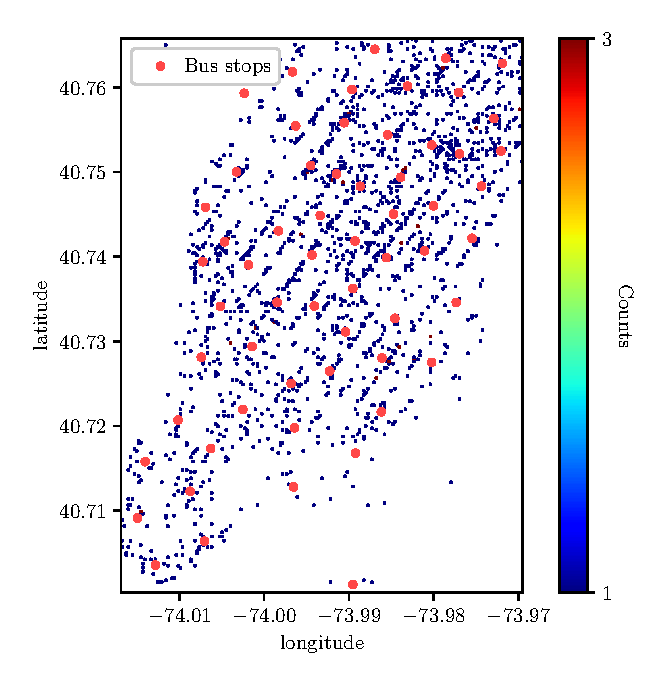
\includegraphics[width=0.5\textwidth]{./data/trips_and_stops_map}}
		\caption{Endpoints density of taxi trips and bus stops}
		\label{fig:clusters}
	\end{center}
	\vskip -5mm
\end{figure}

The heatmap of the endpoints of the taxi trips in figure~\ref{fig:clusters} indicate that mid-town Manhattan, i.e. top right corner of figure, generates the majority of traffic, while Times Square (-73.99, 40.75) is the location with the highest density. As expected, it is evident that the main avenues which run down Manhattan also generate much higher demand than the horizontal, smaller, roads. With the initial 40 bus stops, the 90th percentile of the walking distance from the endpoints to the nearest bus stop was 506$m$ and we had to create 65 stops in order to drop down to 394$m$, i.e. below our threshold of 400$m$. The final location of the 65 bus stops is shown in figure~\ref{fig:clusters} and we observe that they are uniformly distributed on the grid with their density slightly increasing as we approach mid-town Manhattan.

After clustering the bus stops and creating each bus route we are presented with the routes found in figure~\ref{fig:bus_routes}. Even without performing the evaluation step we can observe that some of them are severely inefficient such as the one in the bottom left corner which takes a detour to Brooklyn. Some others are created in such a way that it is faster for the user to get off the bus at an exit and get on the same bus after some stops, i.e. it is faster to get off at stop A, walk from A to B and get on the same bus from B to stop C, than to ride the bus through A-B-C. In addition, we didn't implement connections between the routes so the user is forced to walk in order to catch different buses. We could have expanded each route to traverse bus stops from different routes but it is a trade-off. It would have decreased the duration of trips requiring a bus switch but it would increase the duration of trips that use only one bus.

\begin{figure}[tph]
	\vskip 5mm
	\begin{center}
		\centerline{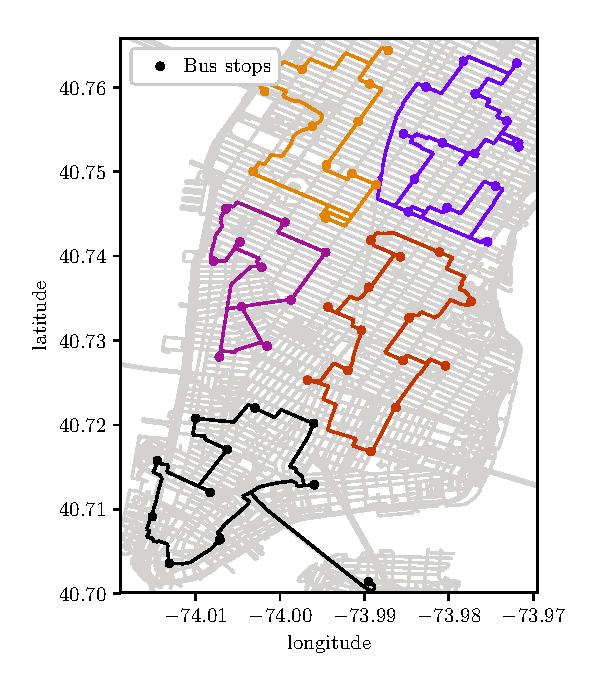
\includegraphics[width=0.5\textwidth]{./data/bus_routes}}
		\caption{Bus routes and their stops}
		\label{fig:bus_routes}
	\end{center}
	\vskip -5mm
\end{figure}

The results of comparing our model's trips' durations to the durations using a taxi \citep{donovan_new_2016} are listed in table~\ref{tab:bus_vs_taxi}. The results are grouped by each trip's Manhattan distance and the performance is calculated as the taxi duration divided by the bus duration. The performance of our model is decreasing as the distance increases and we have an average of 37\%. This can be attributed both to the lower speeds of a bus, especially in Manhattan \citep{edelman_nycs_2017}, but also to the inefficient routes. It is indicative that using our model, 63\% of the total distance was travelled on foot instead of taking a bus. Especially, for small distances, walking was more efficient than riding a bus and in about 50\% of those trips no bus was used. Although we do not take into account the stopping delays at the bus stops, we must mention that we also do not count the waiting time of finding a taxi. However, not implementing a schedule for our model and assuming that there is always a bus available at a bus stop is a major unfair advantage for our model. An example trip is available in appendix \ref{appendix:example_trip}.

The major hindrance in our model is using $k$-means clustering to group the bus stops which results in local circuits. Especially the bottom left route is rendered useless because of the detour. It would have been better to cluster together stops in a straight line even if the distance was longer in order to avoid traversing arcs.

\section{Conclusion}
Our approach utilised the power of open data in order to automate the procedure of building bus transportation networks. The major contribution of this papers is identifying that using $k$-means clustering in order to assign buses to bus stops results in circular routes with low performance. However, a more fair comparison in future attempts would be to fetch the actual travel duration by bus, using the Google Maps API \citep{get_started_|_directions_api_notitle_2018}, since taxis are inherently faster. In addition, it is imperative to create connections between routes and in order to be realistic we have to implement waiting times and use a directed graph to account for one way streets.

\clearpage
\bibliography{project}

\clearpage
\begin{appendices}                               
\section{Example Trip}
\label{appendix:example_trip}
\begin{figure}[h]
	\vskip 5mm
	\begin{center}
		\centerline{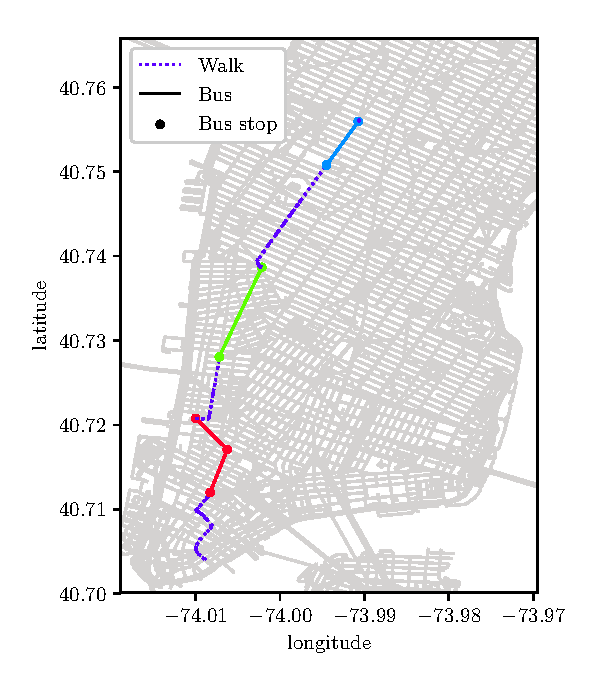
\includegraphics[width=0.5\textwidth]{./data/example_trip}}
		\caption{Trip route example}
		\label{fig:example_trip}
	\end{center}
	\vskip -5mm
\end{figure}
\end{appendices}

\end{document}
